\documentclass[11pt,a4paper]{article}

\usepackage[margin=2.5cm]{geometry}
\usepackage{amsmath,amssymb,amsfonts}
\usepackage{graphicx}
\usepackage{booktabs}
\usepackage{bm}
\usepackage{hyperref}
\usepackage{natbib}

\title{A Short Empirical Study of Hawkes Process Models for Earthquake Occurrences}
\author{Florentin A\bsc{CKER}}
\date{\today}

\begin{document}

\maketitle

\begin{abstract}
We compare a homogeneous Poisson process with marked and unmarked exponential
and power-law Hawkes processes on an earthquake catalogue from the USGS
Earthquake Hazards Program. Models are fitted by maximum likelihood and
evaluated via the time-rescaling theorem. Kolmogorov--Smirnov and chi-squared
tests on the rescaled residuals consistently favour the marked exponential
Hawkes model.
\end{abstract}



\section{Introduction}

Point process models are a standard tool for studying the temporal
structure of earthquake occurrences and quantifying aftershock activity.
The simplest benchmark is a homogeneous Poisson process, which assumes
independent exponentially distributed inter-event times. However,
observed catalogues typically exhibit strong temporal clustering, with
bursts of activity following large events, which motivates the use of
self-exciting Hawkes processes.

In this short note we compare five models on an earthquake catalogue
from the USGS Earthquake Hazards Program: a homogeneous Poisson process,
unmarked and marked exponential and power-law Hawkes processes. Our goal
is to identify a parsimonious specification that captures the observed
clustering and magnitude dependence of aftershock activity, as assessed
by residual diagnostics under the time-rescaling theorem.

\section{Data}

We use an earthquake catalogue retrieved from the United States Geological
Survey (USGS) Earthquake Hazards Program database,\footnote{https://earthquake.usgs.gov/earthquakes/search/}
which provides event times, locations and magnitudes
for earthquakes worldwide. We select earthquakes occurring between
01/01/2025 and 04/05/2026 within the United States of America. The data set
contains $N = 2961$ events over an observation window of approximately
449 days.

For the purpose of this study we ignore spatial information and model only
the temporal occurrence times, treating the catalogue as a one-dimensional
point process on $[t_0, T]$. We centre and scale the times so that $t_0 = 0$
and keep magnitudes in their original units. A lower magnitude cut-off $M_0$
is imposed to ensure approximate completeness of the catalogue.

\section{Models and methods}
\label{sec:analysis}

\subsection{Point process models}

Let $(N_t)_{t\ge 0}$ denote the counting process associated with the
earthquake times $t_1 < \dots < t_N$ on $[0,T]$. All models are
specified through their conditional intensity
$\lambda(t \mid \mathcal{F}_t)$, where $\mathcal{F}_t$ is the history
up to time $t$.

The homogeneous Poisson model assumes a constant intensity
$\lambda(t) \equiv \lambda > 0$, so that the inter-event times are
i.i.d.\ $\mathrm{Exp}(\lambda)$. In contrast, Hawkes processes have the
form
\[
  \lambda(t) = \mu + \sum_{t_i < t} g(t - t_i, M_i),
\]
where $\mu > 0$ is a background rate and $g$ is a triggering kernel.
We consider four Hawkes specifications:
\begin{itemize}
  \item Exponential kernel (unmarked):
    $g(u,M) = \alpha e^{-\beta u} \mathbf{1}_{\{u>0\}}$.
  \item Power-law kernel (unmarked):
    $g(u,M) = K (c+u)^{-p} \mathbf{1}_{\{u>0\}}$.
  \item Marked exponential kernel:
    $g(u,M) = \alpha e^{\gamma (M-M_0)} e^{-\beta u} \mathbf{1}_{\{u>0\}}$.
  \item Marked power-law kernel:
    $g(u,M) = K e^{\gamma (M-M_0)} (c+u)^{-p} \mathbf{1}_{\{u>0\}}$.
\end{itemize}
All parameters are constrained to ensure positivity and stability
(e.g.\ $\alpha/\beta < 1$ in the exponential case).
All parameters are constrained to ensure positivity and stability
(e.g.\ $\alpha/\beta < 1$ in the exponential case, and $p \leq 5$
in the power-law specifications, as larger exponents yield a kernel
decay so rapid that the power-law and exponential specifications
become virtually indistinguishable).

\subsection{Maximum likelihood estimation}

For a given intensity model $\lambda_\theta(t)$ with parameter vector
$\theta$, the log-likelihood of the observed times is
\[
\ell(\theta)
  = \sum_{i=1}^N \log \lambda_\theta(t_i)
    - \int_0^T \lambda_\theta(t)\, \mathrm{d}t.
\]
For the homogeneous Poisson model the MLE is
$\hat{\lambda} = N / (T - t_0)$. For all Hawkes models we evaluate the
log-likelihood numerically and maximise it using the \texttt{scipy.minimize}
routine with a quasi-Newton method and simple box constraints on the
parameters.

\subsection{Residual analysis via time rescaling}

To assess absolute goodness of fit we use Ogata's time-rescaling
theorem. Given a fitted model with intensity $\lambda_{\hat\theta}$, we
compute the integrated intensity
$\Lambda_{\hat\theta}(t) = \int_{0}^{t} \lambda_{\hat\theta}(s)\,
\mathrm{d}s$ and define transformed times
$\tau_i = \Lambda_{\hat\theta}(t_i)$. Under correct specification, the
rescaled gaps $\Delta\tau_i = \tau_i - \tau_{i-1}$ should be i.i.d.\
$\mathrm{Exp}(1)$. We therefore apply Kolmogorov--Smirnov and
chi-squared tests against the $\mathrm{Exp}(1)$ law and compare the
empirical CDFs and densities of the $\Delta\tau_i$ to their theoretical
exponential counterparts. This allows us to check not only relative
fit, but also whether a given model can be regarded as an adequate
description of the data in absolute terms.

\section{Results}
\subsection{Empirical evidence of temporal clustering}
Figure~\ref{fig:ecdf-dt-poisson} compares the empirical CDF of the
inter-event times $\Delta t_i = t_i - t_{i-1}$ with the
$\mathrm{Exp}(\hat\lambda)$ CDF, where $\hat\lambda = N/(T-t_0)$.
The empirical curve lies above the Poisson benchmark near the origin
and below it for intermediate gaps, indicating an excess of very short
inter-event times and a deficit of medium gaps. This pattern is
characteristic of aftershock clustering and already suggests that a
homogeneous Poisson process is inadequate.

\begin{figure}[t]
  \centering
  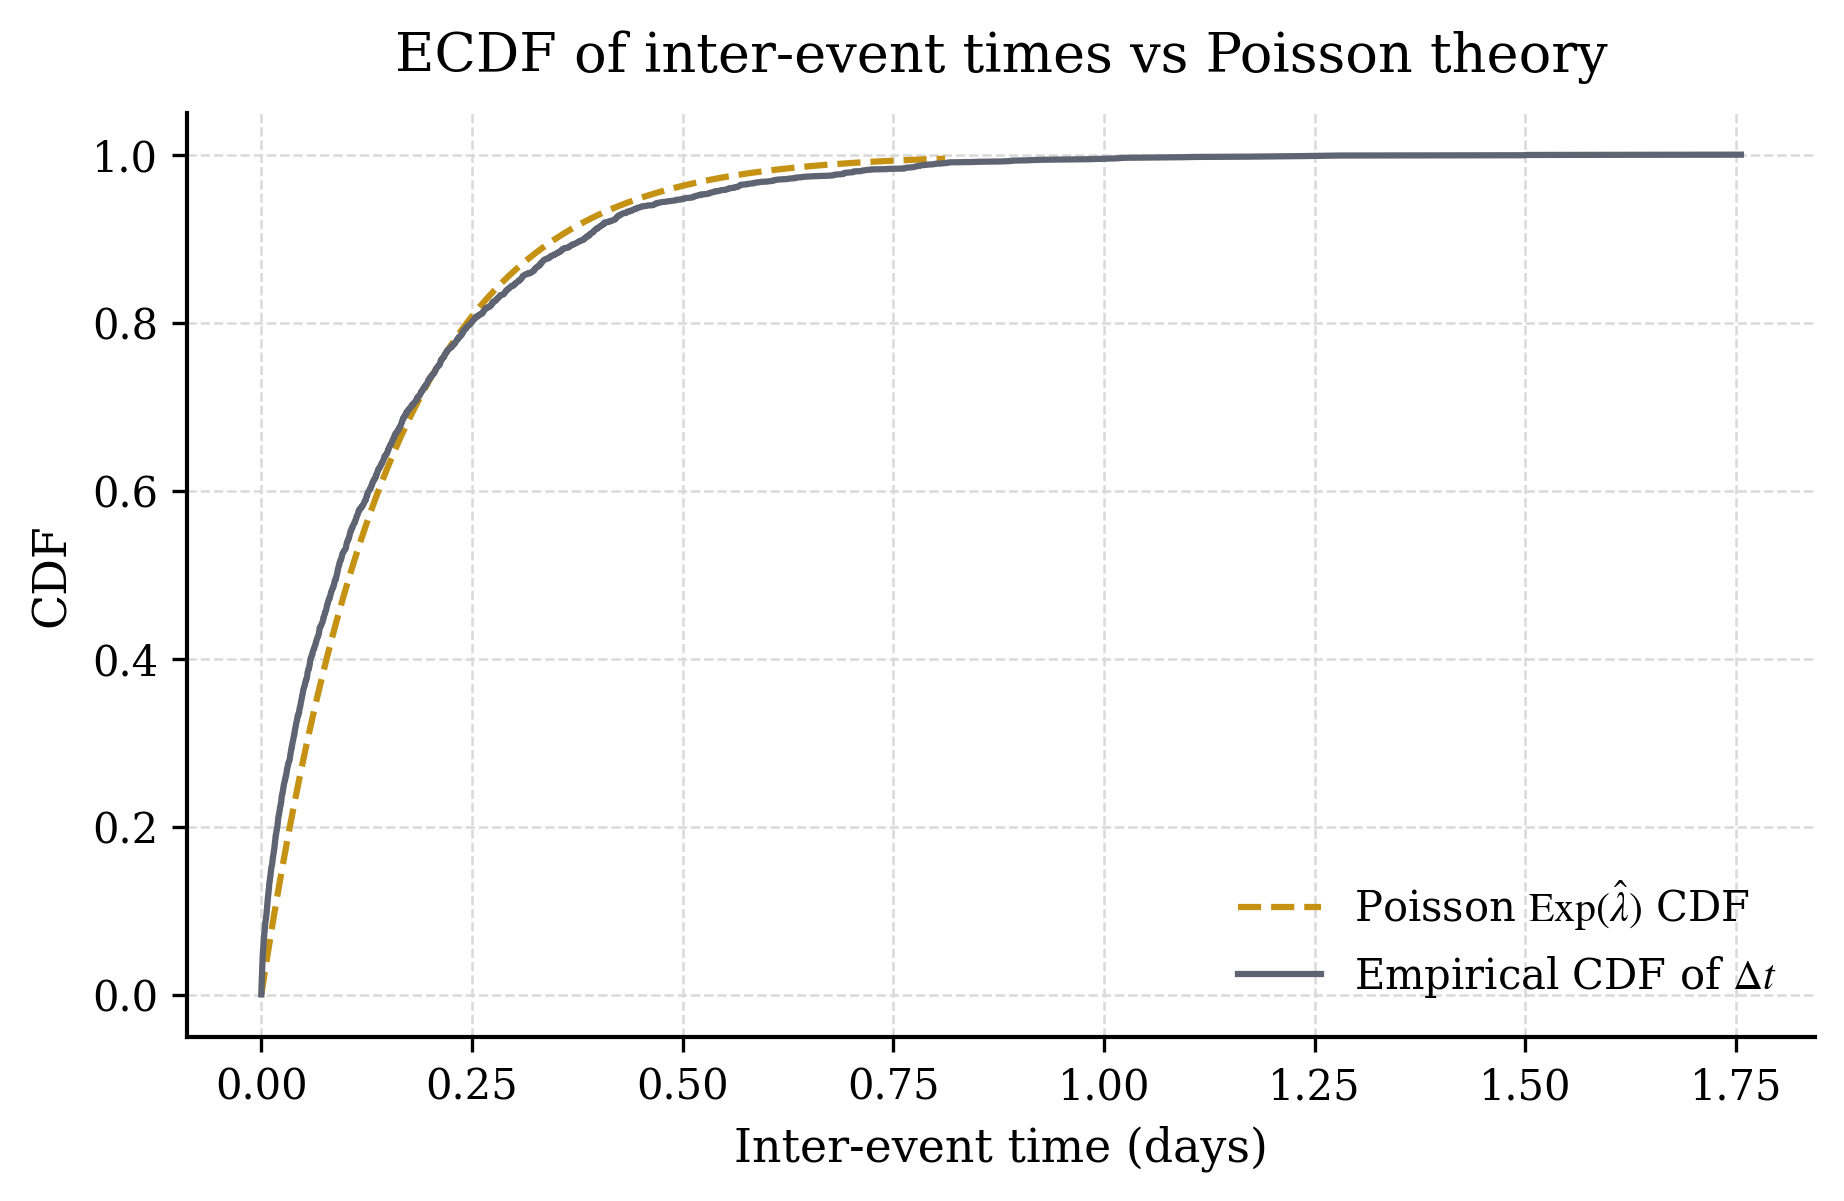
\includegraphics[width=0.8\textwidth]{plots/ecdf_dt_vs_poisson.png}
  \caption{Empirical CDF of $\Delta t_i$ (solid) against the
  $\mathrm{Exp}(\hat\lambda)$ CDF (dashed).}
  \label{fig:ecdf-dt-poisson}
\end{figure}

\subsection{Fitted models}
Table~\ref{tab:params} reports the MLE parameter estimates for all
five models. The Hawkes fits indicate substantial self-excitation, and
the marked models yield $\hat\gamma > 0$, confirming a positive
dependence of triggering strength on magnitude.
Figure~\ref{fig:intensity-full} shows the fitted conditional intensities
for the three main models: the Poisson intensity is constant, whereas
both Hawkes intensities are spiky, with the marked variant producing
sharper peaks after large earthquakes.

\begin{table}[t]
  \centering
  \caption{MLE parameter estimates.}
  \label{tab:params}
  \begin{tabular}{lc}
    \toprule
    Model & Estimates \\
    \midrule
    Poisson &
      $\hat\lambda = 6.59$ \\
    Exponential Hawkes &
      $(\hat\mu,\hat\alpha,\hat\beta) = (5.47, 9.16, 53.98)$ \\
    Power-law Hawkes &
      $(\hat\mu,\hat K,\hat c,\hat p) = (3.30, 0.05, 0.10, 1.50)$ \\
    Marked exp.\ Hawkes &
      $(\hat\mu,\hat\alpha,\hat\beta,\hat\gamma) = (5.52, 5.02, 55.85, 1.12)$ \\
    Marked power-law Hawkes &
      $(\hat\mu,\hat K,\hat c,\hat p,\hat\gamma) = (4.38, 0.067, 0.55, 5.00, 1.09)$ \\
    \bottomrule
  \end{tabular}
\end{table}

\begin{figure}[t]
  \centering
  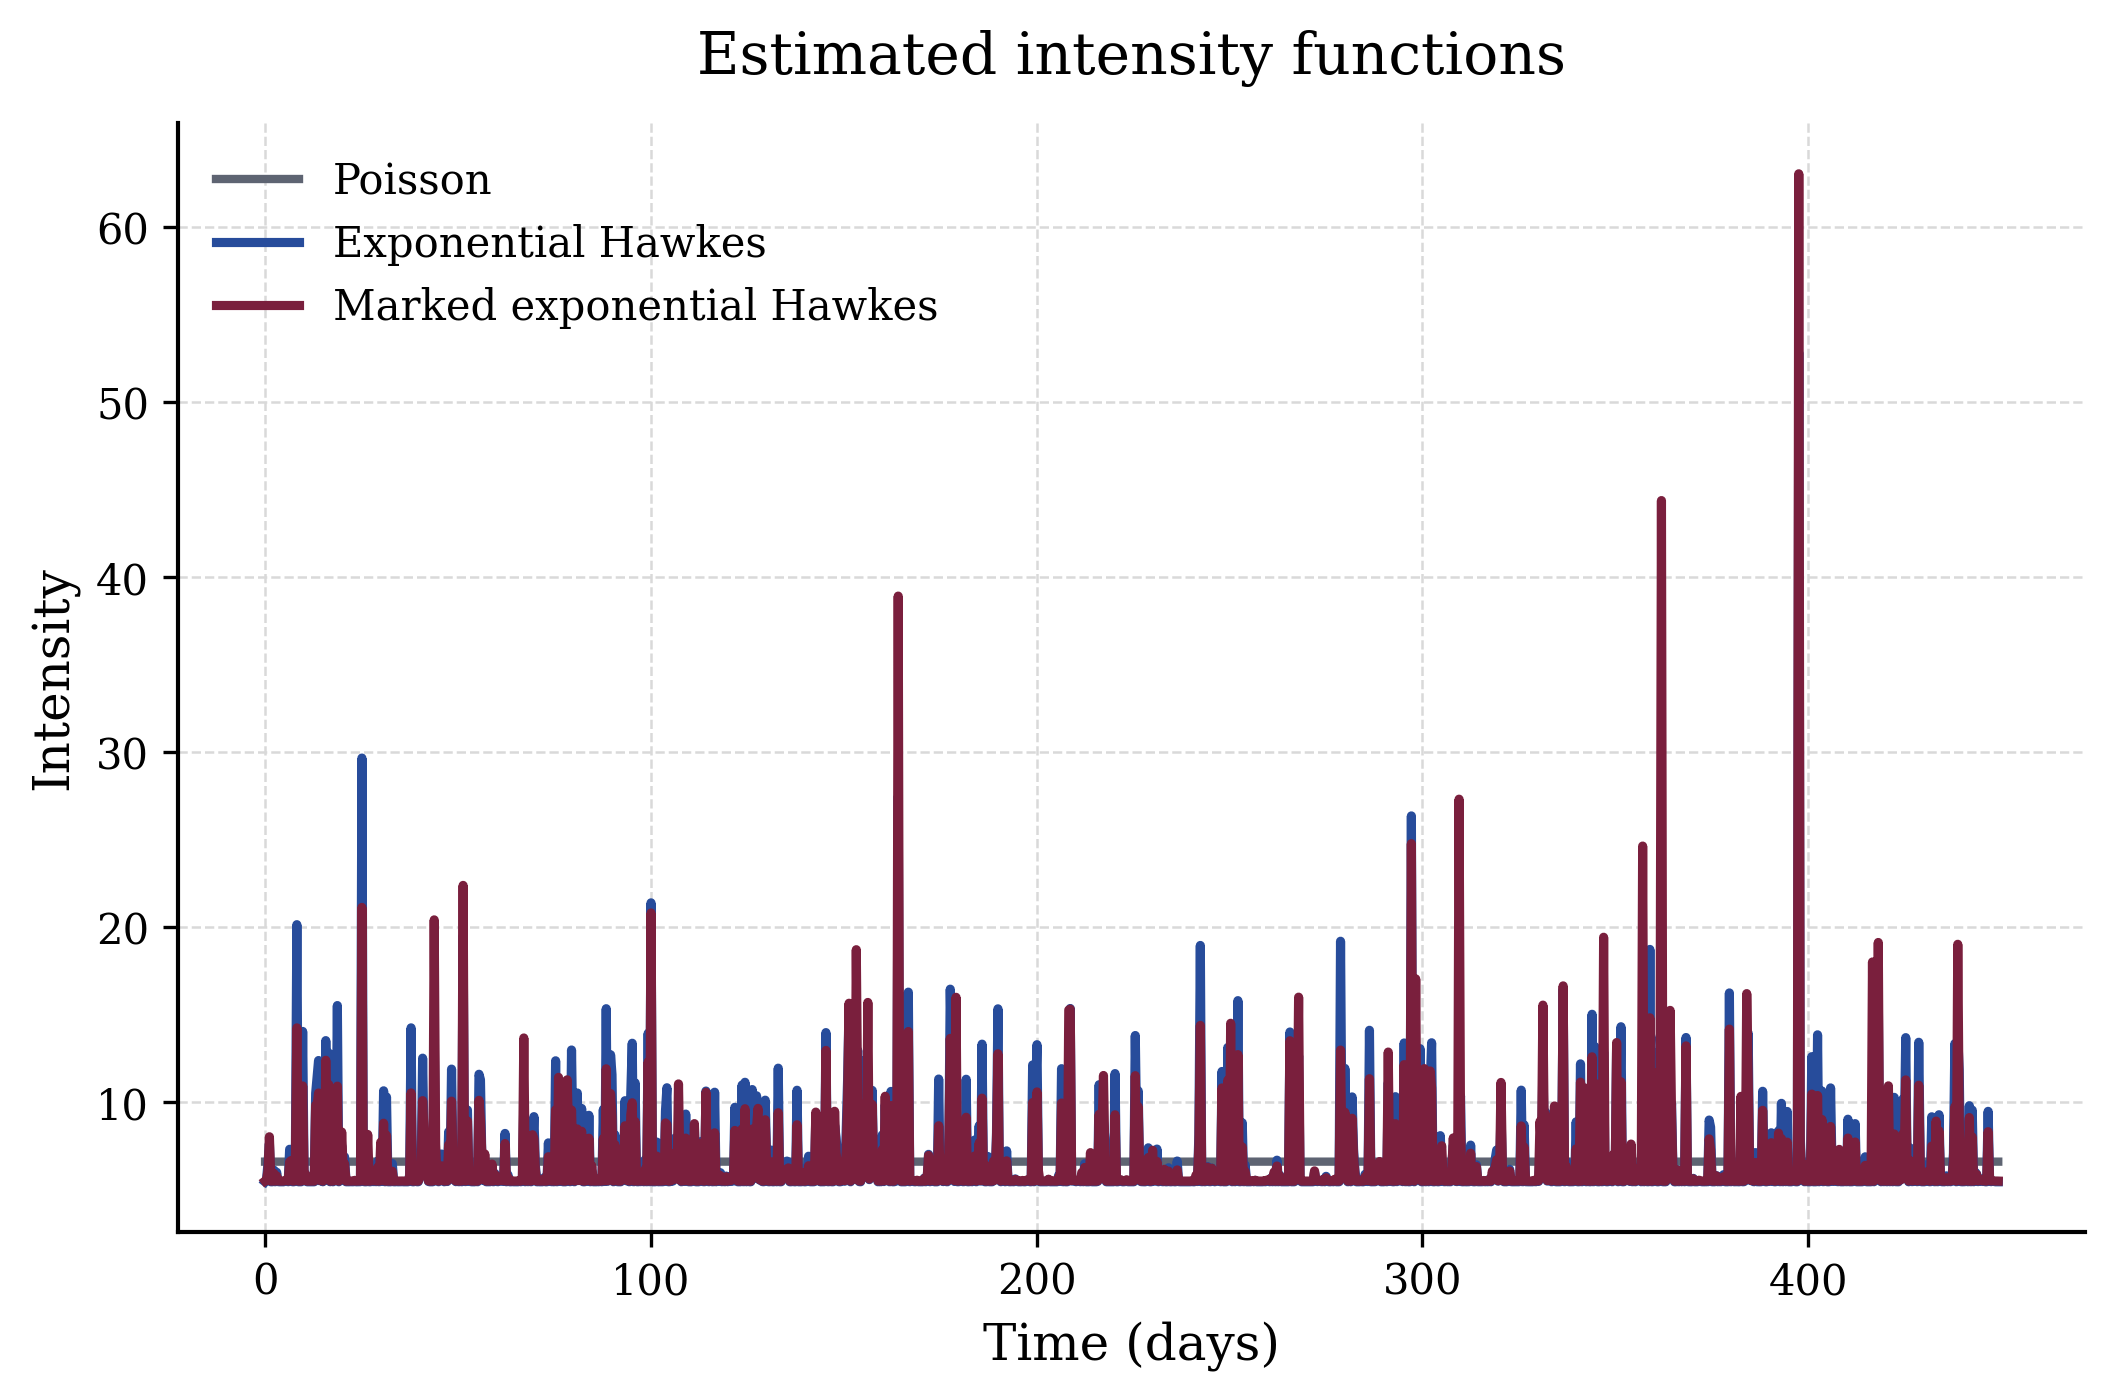
\includegraphics[width=0.8\textwidth]{plots/intensity_curves.png}
  \caption{Estimated conditional intensity functions for the Poisson,
  exponential Hawkes and marked exponential Hawkes models.}
  \label{fig:intensity-full}
\end{figure}

\subsection{Residual diagnostics}
We apply Ogata's time-rescaling theorem: under correct specification,
the rescaled gaps $\Delta\tau_i = \Lambda_{\hat\theta}(t_i) -
\Lambda_{\hat\theta}(t_{i-1})$ should be i.i.d.\ $\mathrm{Exp}(1)$.
The Poisson and power-law Hawkes models are both strongly rejected by
KS and chi-squared tests ($p < 10^{-19}$). The exponential Hawkes model
performs substantially better (KS statistic $0.022$, $p \approx 0.12$),
and the marked exponential Hawkes model provides the best agreement
(KS statistic $0.017$, $p \approx 0.39$; chi-squared $p \approx 0.07$).
Figures~\ref{fig:ks-three} and~\ref{fig:density-three} confirm this
visually: the marked exponential Hawkes residuals are nearly
indistinguishable from the $\mathrm{Exp}(1)$ benchmark, while all
other models show clear discrepancies.

\begin{figure}[t]
  \centering
  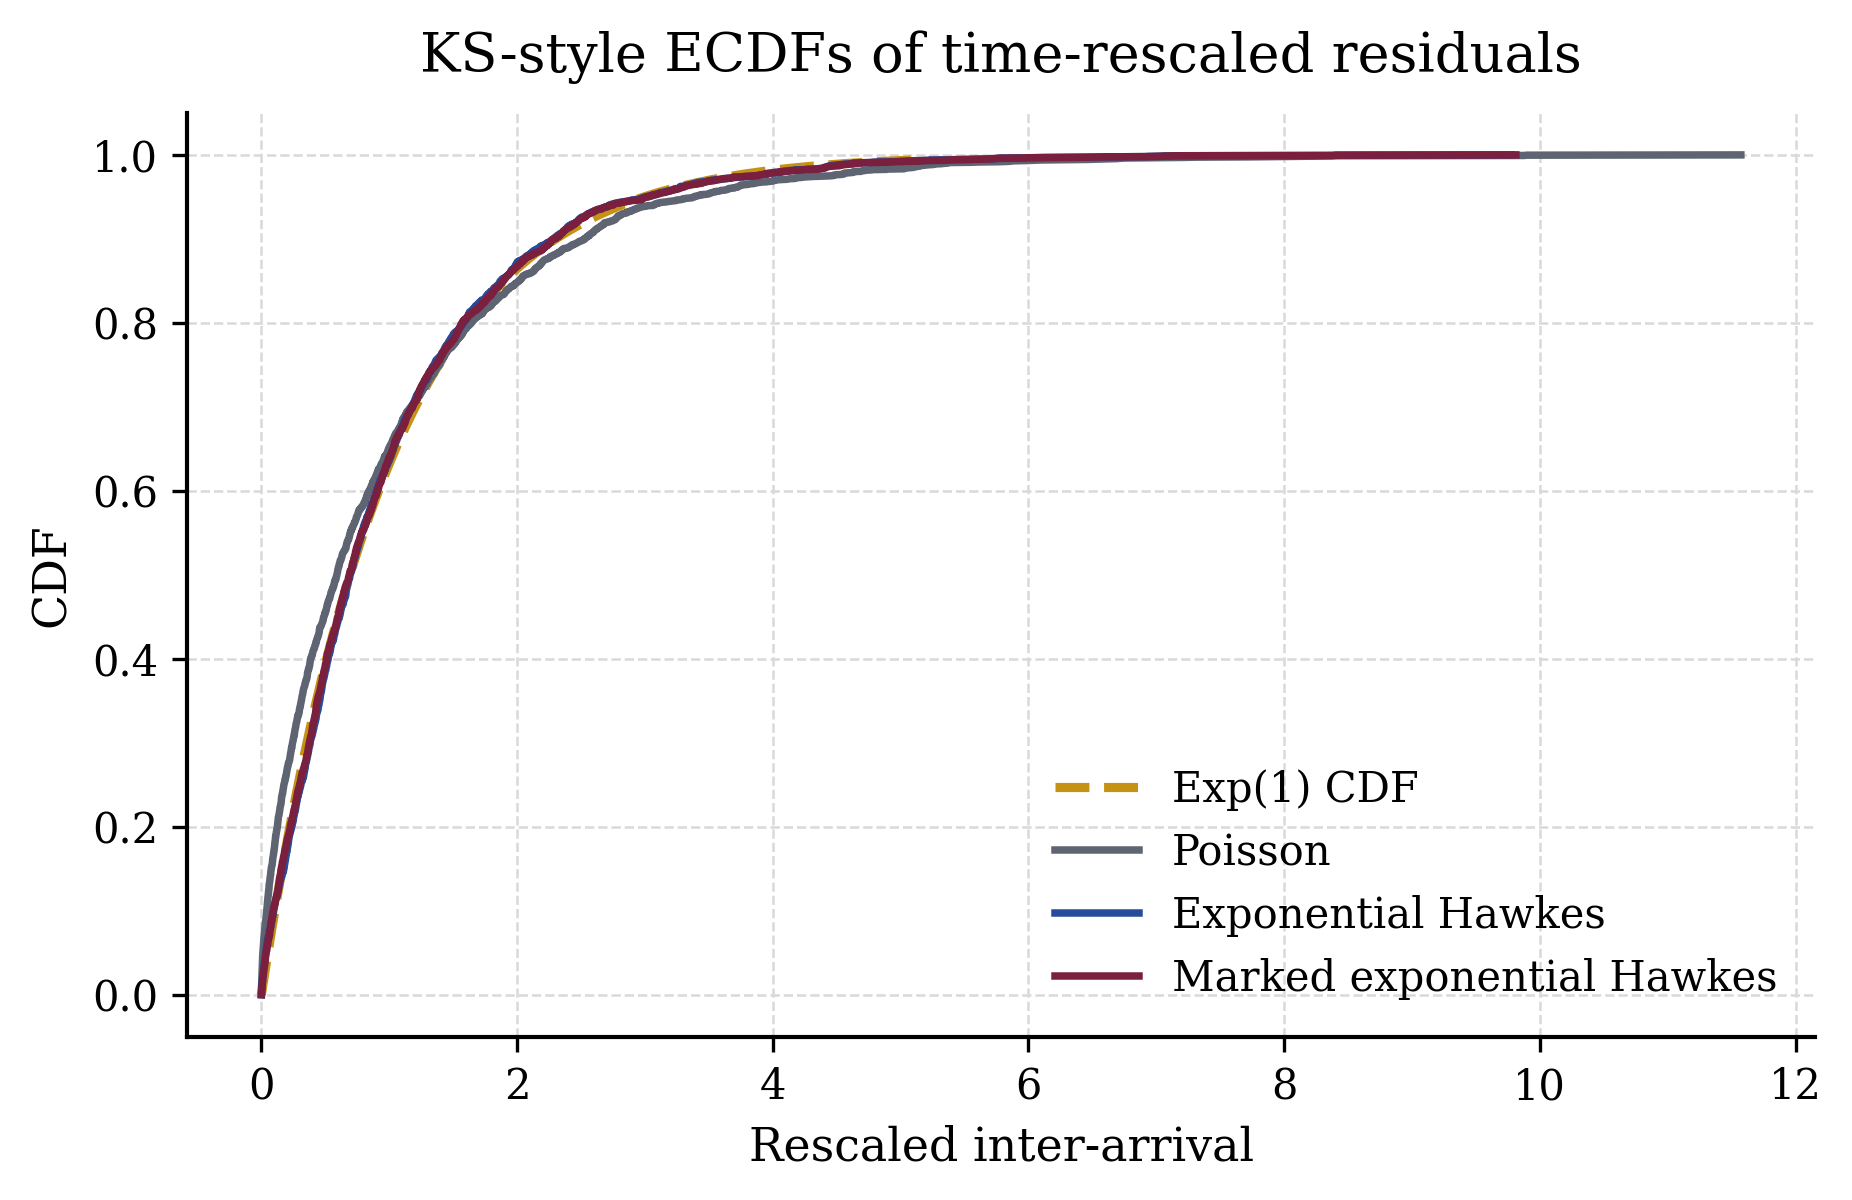
\includegraphics[width=0.8\textwidth]{plots/ks_ecdf_residuals.png}
  \caption{Empirical CDFs of the rescaled inter-arrival times against
  the $\mathrm{Exp}(1)$ CDF (dashed).}
  \label{fig:ks-three}
\end{figure}

\begin{figure}[t]
  \centering
  
\includegraphics[width=0.8\textwidth]{plots/density_residuals.png}
  \caption{Residual densities against the $\mathrm{Exp}(1)$ density
  (dashed).}
  \label{fig:density-three}
\end{figure}

\section{Conclusion}

Using an earthquake catalogue from the USGS database, we compared a
homogeneous Poisson process with several Hawkes process specifications,
including marked and unmarked exponential and power-law kernels. Simple
diagnostics on the raw inter-event times reveal pronounced temporal
clustering that is incompatible with a constant-rate Poisson model.
Residual analyses under the time-rescaling theorem, based on
Kolmogorov--Smirnov and chi-squared tests, point to the marked
exponential Hawkes process as the most adequate representation of the
data: it captures both short-term aftershock clustering and the positive
dependence of triggering intensity on earthquake magnitude, yielding
rescaled inter-arrivals that are approximately $\mathrm{Exp}(1)$.

Several limitations remain. The analysis is purely temporal and ignores
the spatial distribution of events; a space--time Hawkes process would
likely provide a more faithful description of seismicity in the region.
The background rate $\mu$ is assumed constant throughout the observation
window, which may not hold over long periods or across distinct seismic
sequences.




\end{document}
